\documentclass{standalone}
\usepackage{tikz}
\usetikzlibrary{patterns, positioning}
\usepackage[sfdefault]{ClearSans} %% option 'sfdefault' activates Clear Sans as the default text font
\usepackage[T1]{fontenc}

\begin{document}
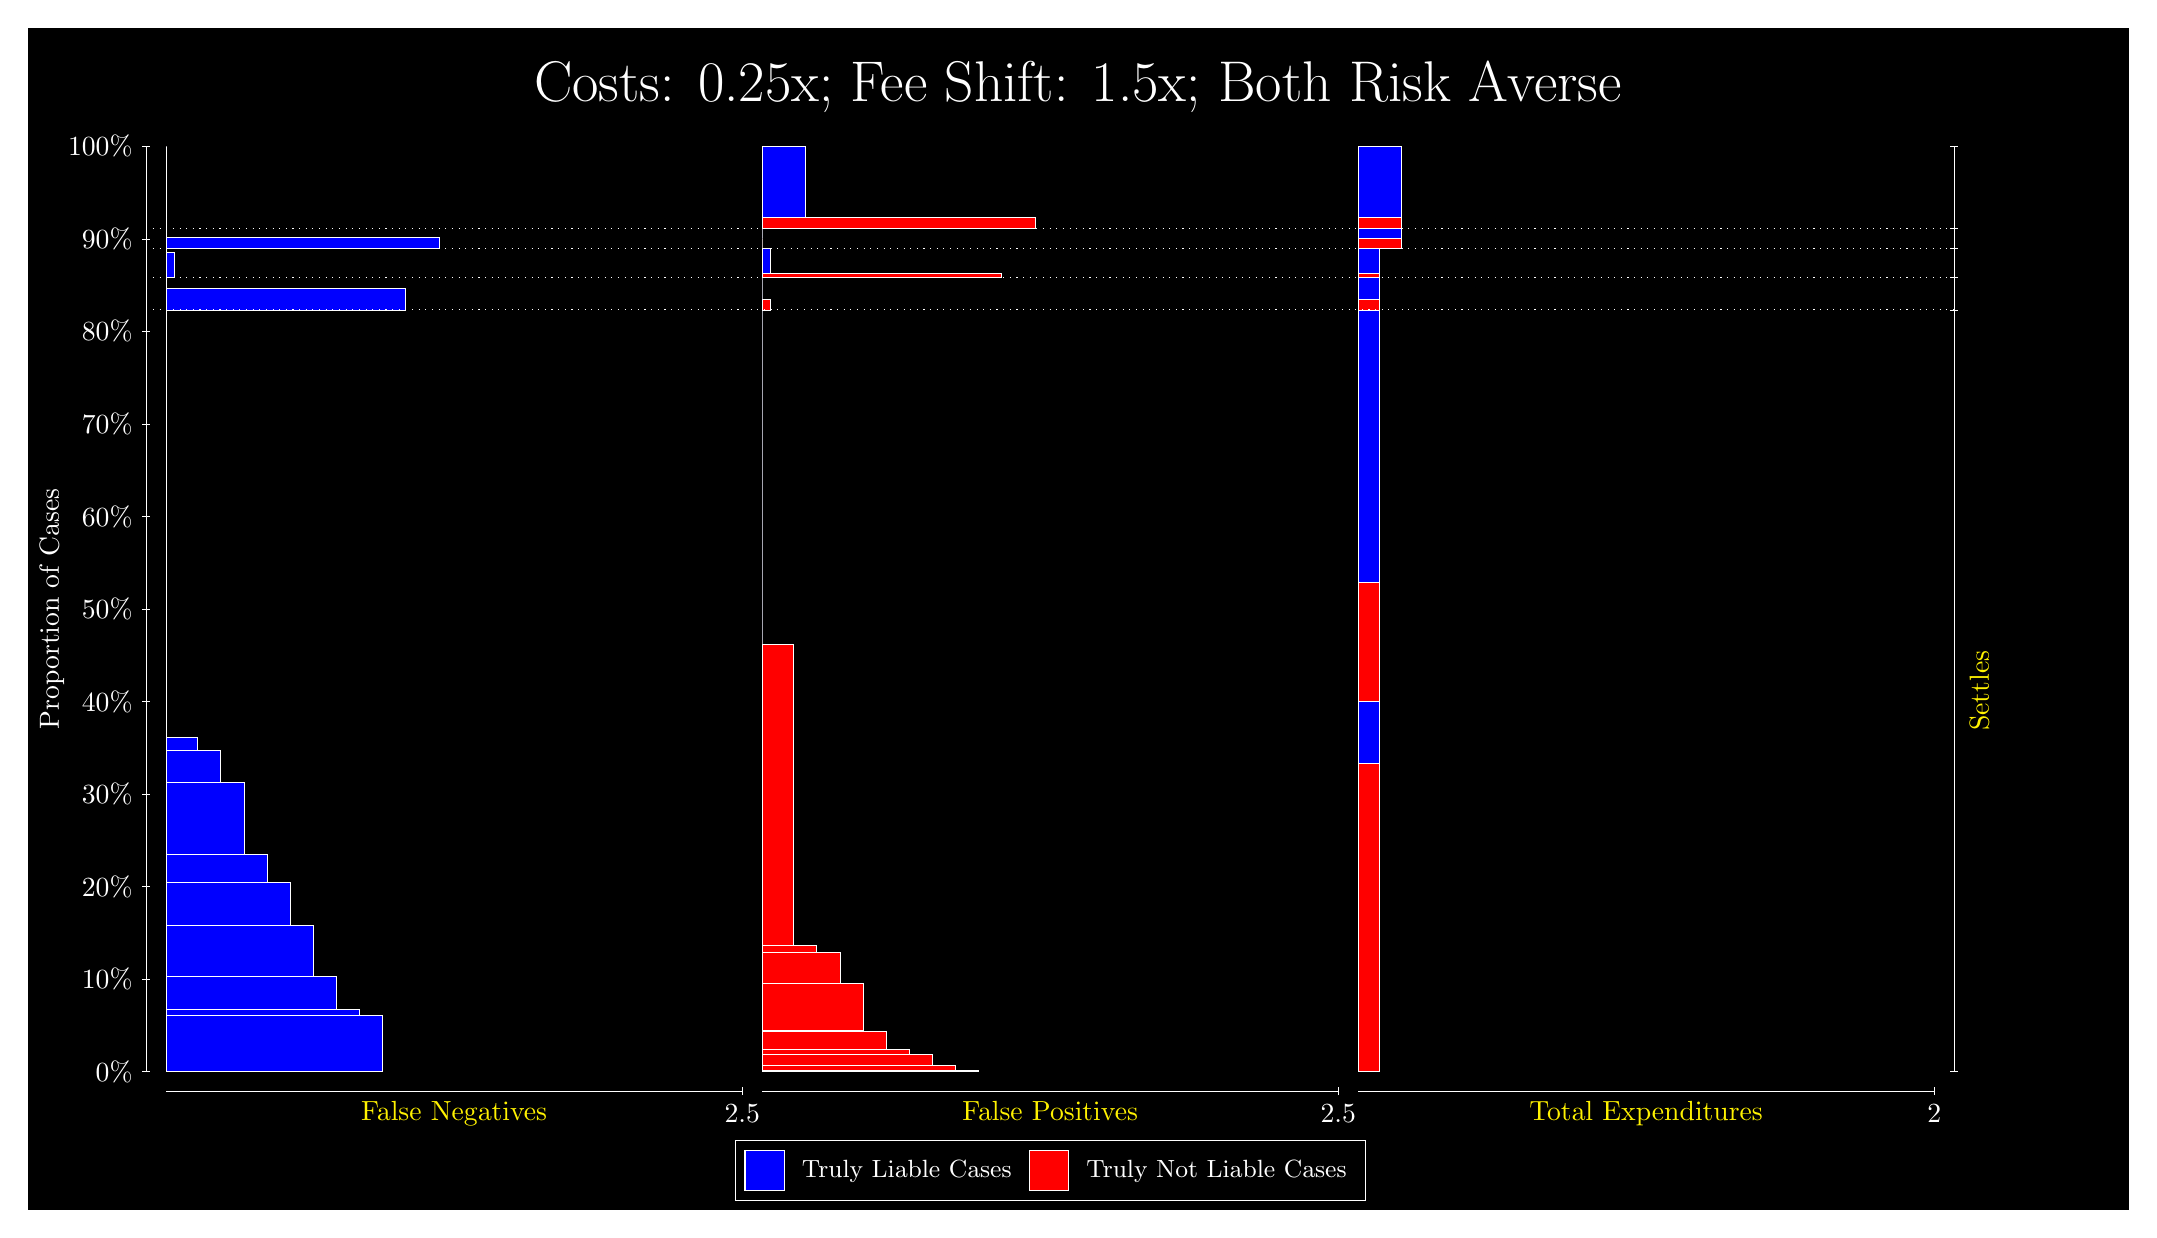
\begin{tikzpicture}
\draw[fill=black] (0,0) rectangle (26.667,15);
\draw[text=white] (0,13.5) rectangle (26.667,15) node[midway] {\huge Costs: 0.25x; Fee Shift: 1.5x; Both Risk Averse};
\draw[white, very thin] (1.5,1.75) -- (1.5,13.5);
\node[rotate=90, text=white, anchor=center] at (0.3, 7.625) {Proportion of Cases};
\draw[white, very thin] (1.45,1.75) -- (1.55,1.75);
\node[text=white, anchor=east] at (1.45, 1.75) {0\%};
\draw[white, very thin] (1.45,2.925) -- (1.55,2.925);
\node[text=white, anchor=east] at (1.45, 2.925) {10\%};
\draw[white, very thin] (1.45,4.1) -- (1.55,4.1);
\node[text=white, anchor=east] at (1.45, 4.1) {20\%};
\draw[white, very thin] (1.45,5.275) -- (1.55,5.275);
\node[text=white, anchor=east] at (1.45, 5.275) {30\%};
\draw[white, very thin] (1.45,6.45) -- (1.55,6.45);
\node[text=white, anchor=east] at (1.45, 6.45) {40\%};
\draw[white, very thin] (1.45,7.625) -- (1.55,7.625);
\node[text=white, anchor=east] at (1.45, 7.625) {50\%};
\draw[white, very thin] (1.45,8.8) -- (1.55,8.8);
\node[text=white, anchor=east] at (1.45, 8.8) {60\%};
\draw[white, very thin] (1.45,9.975) -- (1.55,9.975);
\node[text=white, anchor=east] at (1.45, 9.975) {70\%};
\draw[white, very thin] (1.45,11.15) -- (1.55,11.15);
\node[text=white, anchor=east] at (1.45, 11.15) {80\%};
\draw[white, very thin] (1.45,12.325) -- (1.55,12.325);
\node[text=white, anchor=east] at (1.45, 12.325) {90\%};
\draw[white, very thin] (1.45,13.5) -- (1.55,13.5);
\node[text=white, anchor=east] at (1.45, 13.5) {100\%};

\draw[white, very thin] (24.457,1.75) -- (24.457,13.5);
\draw[white, very thin] (24.407,1.75) -- (24.507,1.75);
\node[anchor=west] at (24.407, 1.75) {};
\draw[white, very thin] (24.407,11.423) -- (24.507,11.423);
\node[anchor=west] at (24.407, 11.423) {};
\draw[white, very thin] (24.407,11.831) -- (24.507,11.831);
\node[anchor=west] at (24.407, 11.831) {};
\draw[white, very thin] (24.407,12.207) -- (24.507,12.207);
\node[anchor=west] at (24.407, 12.207) {};
\draw[white, very thin] (24.407,12.462) -- (24.507,12.462);
\node[anchor=west] at (24.407, 12.462) {};
\draw[white, very thin] (24.407,13.5) -- (24.507,13.5);
\node[anchor=west] at (24.407, 13.5) {};

\draw[white, very thin, fill=blue] (1.75,1.75) rectangle (4.4946,2.4653);
\draw[white, very thin, fill=blue] (1.75,2.4653) rectangle (4.2018,2.5385);
\draw[white, very thin, fill=blue] (1.75,2.5385) rectangle (3.9091,2.9541);
\draw[white, very thin, fill=blue] (1.75,2.9541) rectangle (3.6163,3.6041);
\draw[white, very thin, fill=blue] (1.75,3.6041) rectangle (3.3236,4.1497);
\draw[white, very thin, fill=blue] (1.75,4.1497) rectangle (3.0308,4.5042);
\draw[white, very thin, fill=blue] (1.75,4.5042) rectangle (2.738,5.4255);
\draw[white, very thin, fill=blue] (1.75,5.4255) rectangle (2.4453,5.8277);
\draw[white, very thin, fill=blue] (1.75,5.8277) rectangle (2.1525,5.9931);
\draw[white, very thin, fill=red] (1.75,5.9931) rectangle (1.75,11.423);
\draw[white, very thin, fill=blue] (1.75,11.423) rectangle (4.7873,11.699);
\draw[white, very thin, fill=red] (1.75,11.699) rectangle (1.75,11.831);
\draw[white, very thin, fill=blue] (1.75,11.831) rectangle (1.8598,12.153);
\draw[white, very thin, fill=red] (1.75,12.153) rectangle (1.75,12.207);
\draw[white, very thin, fill=blue] (1.75,12.207) rectangle (5.2265,12.343);
\draw[white, very thin, fill=red] (1.75,12.343) rectangle (1.75,12.462);
\draw[white, very thin, fill=red] (1.75,12.462) rectangle (1.75,12.602);
\draw[white, very thin, fill=blue] (1.75,12.602) rectangle (1.75,13.5);
\draw[white, very thin, fill=red] (9.3189,1.75) rectangle (12.063,1.7711);
\draw[white, very thin, fill=red] (9.3189,1.7711) rectangle (11.771,1.8256);
\draw[white, very thin, fill=red] (9.3189,1.8256) rectangle (11.478,1.9746);
\draw[white, very thin, fill=red] (9.3189,1.9746) rectangle (11.185,2.0305);
\draw[white, very thin, fill=red] (9.3189,2.0305) rectangle (10.892,2.2647);
\draw[white, very thin, fill=red] (9.3189,2.2647) rectangle (10.6,2.2704);
\draw[white, very thin, fill=red] (9.3189,2.2704) rectangle (10.6,2.8769);
\draw[white, very thin, fill=red] (9.3189,2.8769) rectangle (10.307,3.2669);
\draw[white, very thin, fill=red] (9.3189,3.2669) rectangle (10.014,3.348);
\draw[white, very thin, fill=red] (9.3189,3.348) rectangle (9.7214,7.1797);
\draw[white, very thin, fill=blue] (9.3189,7.1797) rectangle (9.3189,11.423);
\draw[white, very thin, fill=red] (9.3189,11.423) rectangle (9.4287,11.555);
\draw[white, very thin, fill=blue] (9.3189,11.555) rectangle (9.3189,11.831);
\draw[white, very thin, fill=red] (9.3189,11.831) rectangle (12.356,11.885);
\draw[white, very thin, fill=blue] (9.3189,11.885) rectangle (9.4287,12.207);
\draw[white, very thin, fill=red] (9.3189,12.207) rectangle (9.3189,12.327);
\draw[white, very thin, fill=blue] (9.3189,12.327) rectangle (9.3189,12.462);
\draw[white, very thin, fill=red] (9.3189,12.462) rectangle (12.795,12.602);
\draw[white, very thin, fill=blue] (9.3189,12.602) rectangle (9.8678,13.5);
\draw[white, very thin, fill=red] (16.888,1.75) rectangle (17.162,5.6627);
\draw[white, very thin, fill=blue] (16.888,5.6627) rectangle (17.162,6.4512);
\draw[white, very thin, fill=red] (16.888,6.4512) rectangle (17.162,7.9681);
\draw[white, very thin, fill=blue] (16.888,7.9681) rectangle (17.162,11.423);
\draw[white, very thin, fill=red] (16.888,11.423) rectangle (17.162,11.555);
\draw[white, very thin, fill=blue] (16.888,11.555) rectangle (17.162,11.831);
\draw[white, very thin, fill=red] (16.888,11.831) rectangle (17.162,11.885);
\draw[white, very thin, fill=blue] (16.888,11.885) rectangle (17.162,12.207);
\draw[white, very thin, fill=red] (16.888,12.207) rectangle (17.437,12.327);
\draw[white, very thin, fill=blue] (16.888,12.327) rectangle (17.437,12.462);
\draw[white, very thin, fill=red] (16.888,12.462) rectangle (17.437,12.602);
\draw[white, very thin, fill=blue] (16.888,12.602) rectangle (17.437,13.5);
\draw[white, dotted] (1.5,11.423) -- (24.457,11.423);
\draw[white, dotted] (1.5,11.831) -- (24.457,11.831);
\draw[white, dotted] (1.5,12.207) -- (24.457,12.207);
\draw[white, dotted] (1.5,12.462) -- (24.457,12.462);
\draw[white, very thin] (1.75,1.5) -- (9.0689,1.5);
\node[text=yellow, anchor=north] at (5.4094, 1.5) {False Negatives};
\draw[white, very thin] (9.0689,1.45) -- (9.0689,1.55);
\node[text=white, anchor=north] at (9.0689, 1.45) {2.5};

\draw[white, very thin] (9.3189,1.5) -- (16.638,1.5);
\node[text=yellow, anchor=north] at (12.978, 1.5) {False Positives};
\draw[white, very thin] (16.638,1.45) -- (16.638,1.55);
\node[text=white, anchor=north] at (16.638, 1.45) {2.5};

\draw[white, very thin] (16.888,1.5) -- (24.207,1.5);
\node[text=yellow, anchor=north] at (20.547, 1.5) {Total Expenditures};
\draw[white, very thin] (24.207,1.45) -- (24.207,1.55);
\node[text=white, anchor=north] at (24.207, 1.45) {2};

\node[text=yellow, centered, rotate=90] at (24.777, 6.5864) {Settles};





\draw (12.978300999999998,1.5) node[draw=none] (baseCoordinate) {};
\begin{scope}[align=center]
        \matrix[scale=0.5, draw=white, below=0.5cm of baseCoordinate, nodes={draw}, column sep=0.1cm]{
            \node[rectangle, draw, minimum width=0.5cm, minimum height=0.5cm, fill=blue] {}; &
            \node[draw=none, font=\small, text=white] (B) {Truly Liable Cases}; &
            \node[rectangle, draw, minimum width=0.5cm, minimum height=0.5cm, fill=red] {}; &
            \node[draw=none, font=\small, text=white] (B) {Truly Not Liable Cases}; \\
            };
\end{scope}

\end{tikzpicture}
\end{document}